\documentclass[aps, prc, twocolumn, reprint]{revtex4-1}

\usepackage{amsmath}
\usepackage{mathtools}
\usepackage{amsfonts}
\usepackage{url}
\usepackage{xspace}
\usepackage{siunitx}
\usepackage[usenames,dvipsnames]{xcolor}
\usepackage{float}
\usepackage[caption=false]{subfig}
\usepackage{framed}

\frenchspacing

% Defined macros

\DeclareMathOperator{\csch}{csch}
\DeclareMathOperator{\sech}{sech}

\newcommand{\degree}[0]{\ensuremath{^\circ}\xspace}
\renewcommand{\implies}{\Rightarrow}
\newcommand{\eval}[1]{\ensuremath{\left<#1\right>}}
\newcommand{\ket}[1]{\ensuremath{\left| #1 \right>}}
\newcommand{\bra}[1]{\ensuremath{\left< #1 \right|}}
\newcommand{\mel}[3]{\ensuremath{\left<#1 \right|\! #2 \!\left| #3 \right>}}
\newcommand{\proj}[2]{\ensuremath{\left<#1 \middle| #2 \right>}}

\newcommand{\pmat}[1]{\ensuremath{\begin{pmatrix}#1\end{pmatrix}}}

\newcommand{\pder}[2]{\ensuremath{\frac{\partial #1}{\partial #2}}}
\newcommand{\ppder}[2]{\ensuremath{\frac{\partial^2 #1}{\partial #2^2}}}
\newcommand{\ppmder}[3]{\ensuremath{\frac{\partial^2 #1}{\partial #2 \partial #3}}}

\newcommand{\pderc}[3]{\ensuremath{\left( \frac{\partial #1}{\partial #2} \right)_{\!\!#3}}}
\newcommand{\ppmderc}[4]{\ensuremath{\left( \frac{\partial^2 #1}{\partial #2 \partial #3} \right)_{\!\!#4}}}

\newcommand{\nuc}[2]{${}^{#1}\text{#2}$}

\newcommand{\fresco}[0]{\textsc{Fresco}\xspace}


\begin{document}

\title{PHY 982 Homework 2: Elastic scattering and optical models}
\author{Josh Bradt}
\author{Chris Izzo}
\date{April 9, 2015}

\maketitle

\section{Elastic scattering calculations}

	We chose to use the nucleus \nuc{100}{Mo} for our target. This nucleus has 42 protons and 58 neutrons. As an even-even nucleus, this target has a ground state of $0^+$.

	\subsection{Pure Coulomb potential}

	We began by running \fresco for elastic scattering of protons at \SI{5}{MeV} and \SI{50}{MeV}. We did this for a point-like potential with a Coulomb radius of \SI{0.001}{fm} and a finite potential with a Coulomb radius of \SI{1.220}{fm}. We chose the second value from the previous homework assignment. Fig.~\ref{fig:protons_nonuc} shows the differential cross sections of these reactions as a ratio to the Rutherford cross sections. We can see that the ratio to Rutherford is approximately 1.0 for all angles for the scattering off of the point-like potential. This is because a point-like potential produces pure Coulomb scattering. For the finite-radius potentials, we found that the ratio to Rutherford is still 1.0 for the low-energy scattering. This is because the low-energy proton does not penetrate beyond the Coulomb radius. The higher-energy proton, on the other hand, penetrates beyond the Coulomb radius and sees that the potential is different from charge concentrated at a point. This explains why the \SI{50}{MeV} proton scattering off of the finite potential produces a cross section that is different from Rutherford, while the others do not.

	Next, we repeated this analysis with neutrons instead of protons. This gave us the elastic scattering cross sections shown in Fig.~\ref{fig:neutrons_nonuc}. As we can see, the scattering cross section is very small. This is because the neutrons are neutral and shouldn't interact with the Coulomb potential. 

	\begin{figure}[bt]
		\centering
		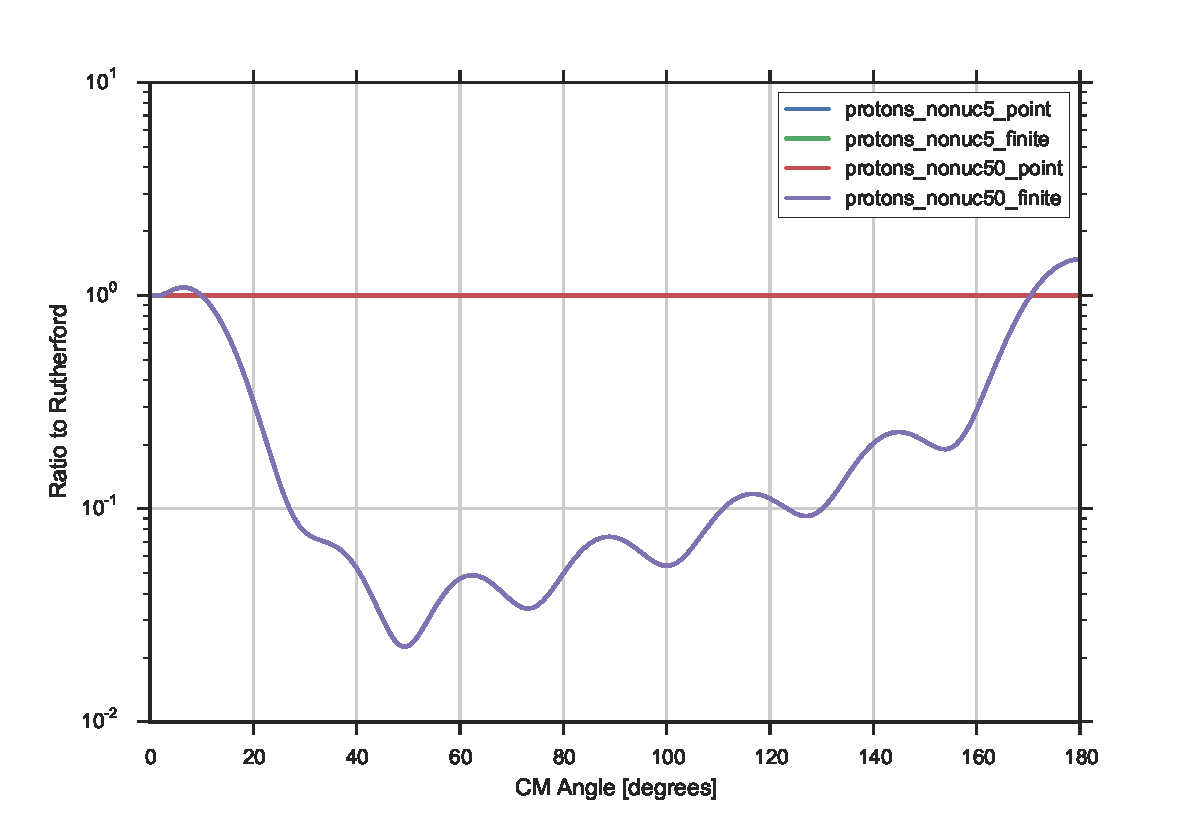
\includegraphics[width=\columnwidth]{{images/protons_nonuc.pdf}}
		\caption{Elastic scattering cross sections for protons on \nuc{100}{Mo} at \SI{5}{MeV} and \SI{50}{MeV} for point-like and finite-radius potentials. This does not include a nuclear potential.}
		\label{fig:protons_nonuc}
	\end{figure}

	\begin{figure}[tb]
		\centering
		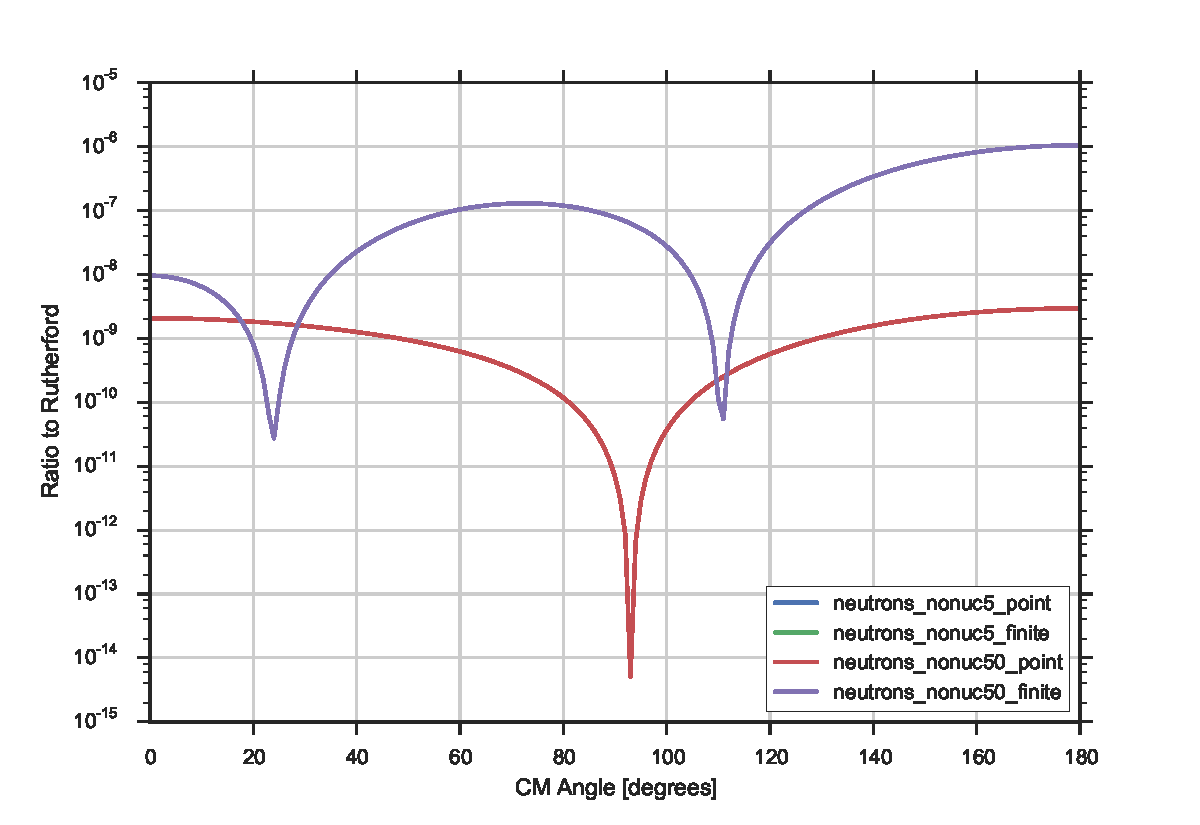
\includegraphics[width=\columnwidth]{{images/neutrons_nonuc.pdf}}
		\caption{Elastic scattering cross sections for neutrons on \nuc{100}{Mo} at \SI{5}{MeV} and \SI{50}{MeV} for point-like and finite-radius potentials. This does not include a nuclear potential.}
		\label{fig:neutrons_nonuc}
	\end{figure}

	\subsection{Nuclear potential}

	Next, we added a nuclear potential. We used a global optical potential of Woods-Saxon shape with parameters from Koning and Delaroche. \cite{Koning2003} We did this for both neutrons and protons. The angular distributions are shown in Fig.~\ref{fig:nuc_all}.

	We can see the following things:
	\begin{enumerate}
		\item For protons at low energy, the scattering cross sections are very close to Rutherford. This is because the low-energy proton does not probe beyond the Coulomb barrier.

		\item As before, the high-energy protons penetrate the Coulomb barrier. This leads to a more complex angular distribution since the proton sees the internal structure of the nucleus.

		\item For both energies, the neutrons probe the nuclear potential. This is because they are not affected by Coulomb repulsion. We also see that there is less scattering to backwards angles for the higher-energy neutrons.
	\end{enumerate}

	\begin{figure}[tb]
		\centering
		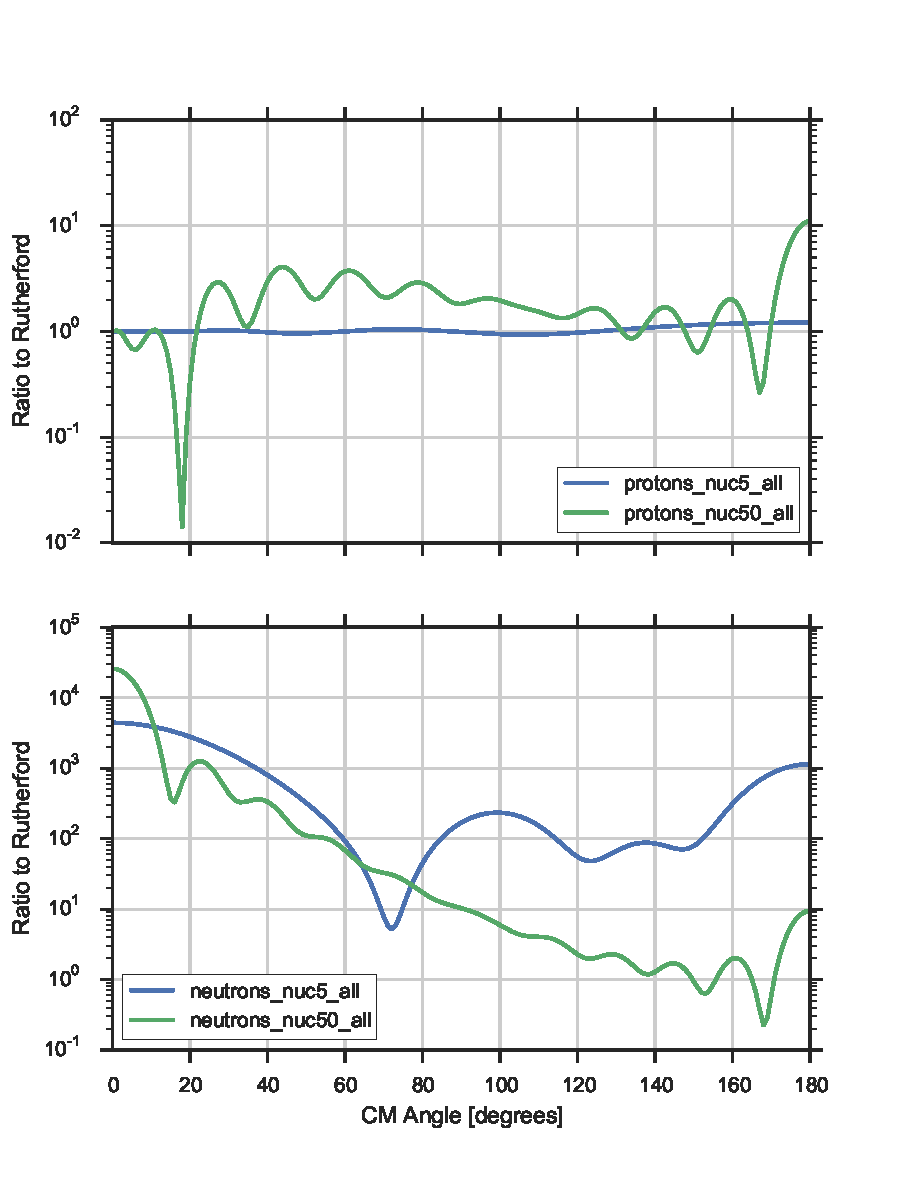
\includegraphics[width=\columnwidth]{{images/nuc_all.pdf}}
		\caption{Elastic scattering cross sections on \nuc{100}{Mo} with a volume nuclear potential for protons (top) and neutrons (bottom) at \SI{5}{MeV} and \SI{50}{MeV}.}
		\label{fig:nuc_all}
	\end{figure}

	\subsection{Contribution of the imaginary part}

	For comparison, we removed the imaginary volume component of the Woods-Saxon nuclear optical potential and examined the behavior of the real part alone. This is shown for both protons and neutrons in Fig.~\ref{fig:nuc_real}. This result looks different from Fig.~\ref{fig:nuc_all} because after removing the imaginary part of the potential, we are no longer accounting for exit channels other than elastic scattering.

	If we compare the $S$ matrices in these two cases, we find that the modulus of the $S$ matrix is 1 for each partial wave in the case of the real potential, as expected. When we add in the imaginary part, the $S$ matrices no longer have a modulus of 1. This indicates that some of the outgoing flux is being absorbed by the imaginary part of the potential. This is shown in Fig~\ref{fig:smat}.

	\begin{figure}[t]
		\centering
		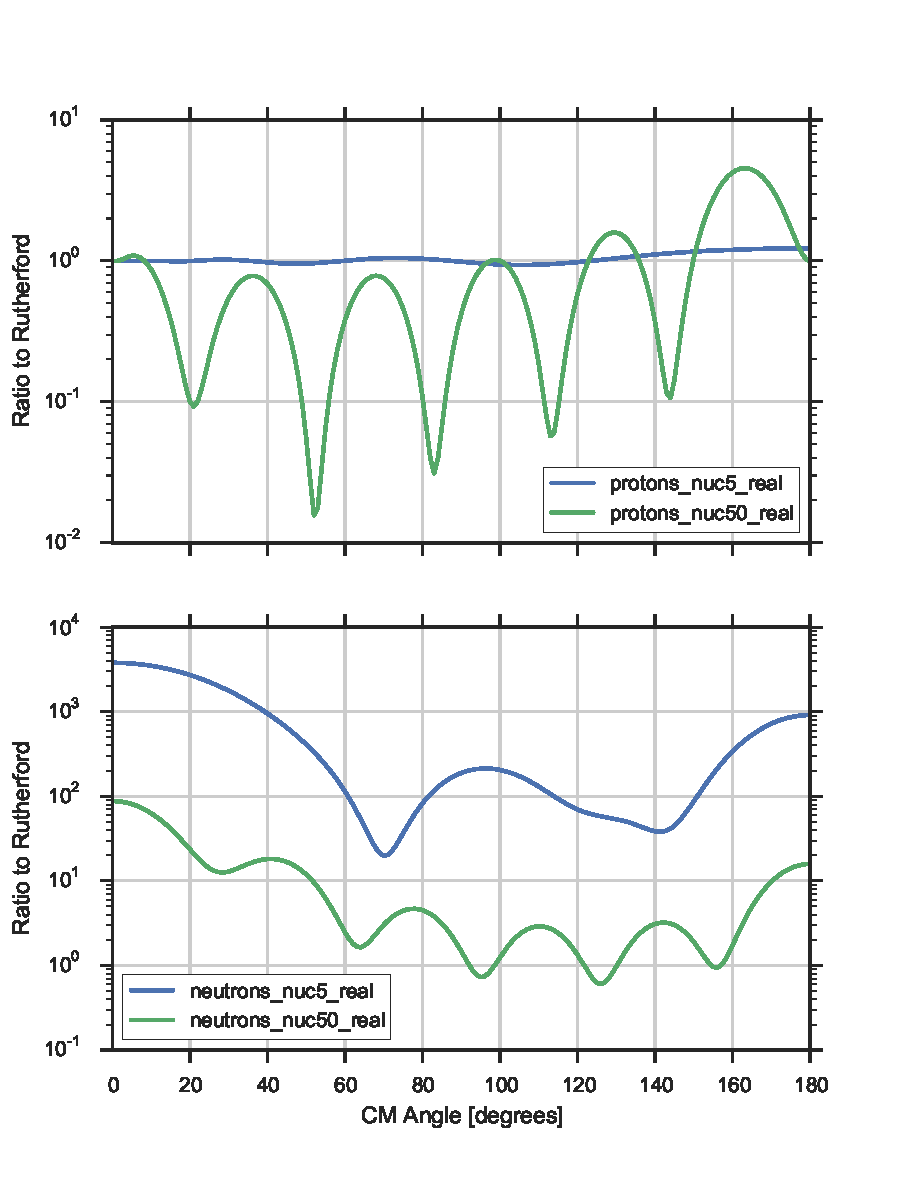
\includegraphics[width=\columnwidth]{{images/nuc_real.pdf}}
		\caption{Elastic scattering cross sections on \nuc{100}{Mo} with only the real component of the volume nuclear potential. This is shown for protons (top) and neutrons (bottom) at \SI{5}{MeV} and \SI{50}{MeV}.}
		\label{fig:nuc_real}
	\end{figure}

	\begin{figure}[tb]
		\centering
		\begin{framed}
		\centering
		\footnotesize
		\begin{verbatim}
			-0.1406733863 -0.9900560582  0  0.5  0.5 : S(L,J,JT)
			-0.9950493561  0.0993819851  1  0.5  0.5 : S(L,J,JT)
			-0.4883262722  0.8726611324  2  1.5  1.5 : S(L,J,JT)
			-0.9950493561  0.0993819851  1  1.5  1.5 : S(L,J,JT)
			-0.4883262722  0.8726611324  2  2.5  2.5 : S(L,J,JT)

			-0.0578241233 -0.4368748881  0  0.5  0.5 : S(L,J,JT)
			-0.4404722371  0.0377326911  1  0.5  0.5 : S(L,J,JT)
			-0.2212677416  0.3878465564  2  1.5  1.5 : S(L,J,JT)
			-0.4404722371  0.0377326911  1  1.5  1.5 : S(L,J,JT)
			-0.2212677416  0.3878465564  2  2.5  2.5 : S(L,J,JT)
		\end{verbatim}
		\end{framed}
		\caption{$S$ matrix elements from \fresco. This is the raw output from the file \texttt{fort.7} for \SI{50}{MeV} protons. The lines above the gap are for the interaction with only the real part, while the lines below the gap are for the interaction with both real and complex parts. It is clear that the moduli of the upper lines are 1.}
		\label{fig:smat}
	\end{figure}

	% \begin{table}[tb]
	% 	\centering
	% 	\begin{ruledtabular}
	% 	\begin{tabular}{c c c c c c}
	% 		  -0.1406733863 & -0.9900560582  &   0  & 0.5  & 0.5 & : S(L,J,JT) \\
	% 		  -0.9950493561 &  0.0993819851  &   1  & 0.5  & 0.5 & : S(L,J,JT) \\
	% 		  -0.4883262722 &  0.8726611324  &   2  & 1.5  & 1.5 & : S(L,J,JT) \\
	% 		  -0.9950493561 &  0.0993819851  &   1  & 1.5  & 1.5 & : S(L,J,JT) \\
	% 		  -0.4883262722 &  0.8726611324  &   2  & 2.5  & 2.5 & : S(L,J,JT) \\
	% 		\colrule
	% 		  -0.0578241233 & -0.4368748881  &   0 &  0.5 &  0.5  & : S(L,J,JT) \\
	% 		  -0.4404722371 &  0.0377326911  &   1 &  0.5 &  0.5  & : S(L,J,JT) \\
	% 		  -0.2212677416 &  0.3878465564  &   2 &  1.5 &  1.5  & : S(L,J,JT) \\
	% 		  -0.4404722371 &  0.0377326911  &   1 &  1.5 &  1.5  & : S(L,J,JT) \\
	% 		  -0.2212677416 &  0.3878465564  &   2 &  2.5 &  2.5  & : S(L,J,JT) \\
	% 	\end{tabular}
	% 	\end{ruledtabular}
	% 	\caption{$S$ matrix elements from \fresco. This is the raw output from the file \texttt{fort.7} for \SI{50}{MeV} protons. The lines above the horizontal rule are for the interaction with only the real part, while the lines below the rule are for the interaction with both real and complex parts. It is clear that the moduli of the upper lines are 1.}
	% 	\label{tab:smat}
	% \end{table}

	\subsection{Increasing the radius}

	Then, we tried increasing the radius parameter in the optical potential and the Coulomb potential to \SI{10}{fm}. We found that it greatly increased the number of oscillations in the graph and increased the total cross section. This is what we expected because making the target larger should increase the cross section. The results are shown in Fig.~\ref{fig:big_r}.

	\begin{figure}[tb]
		\centering
		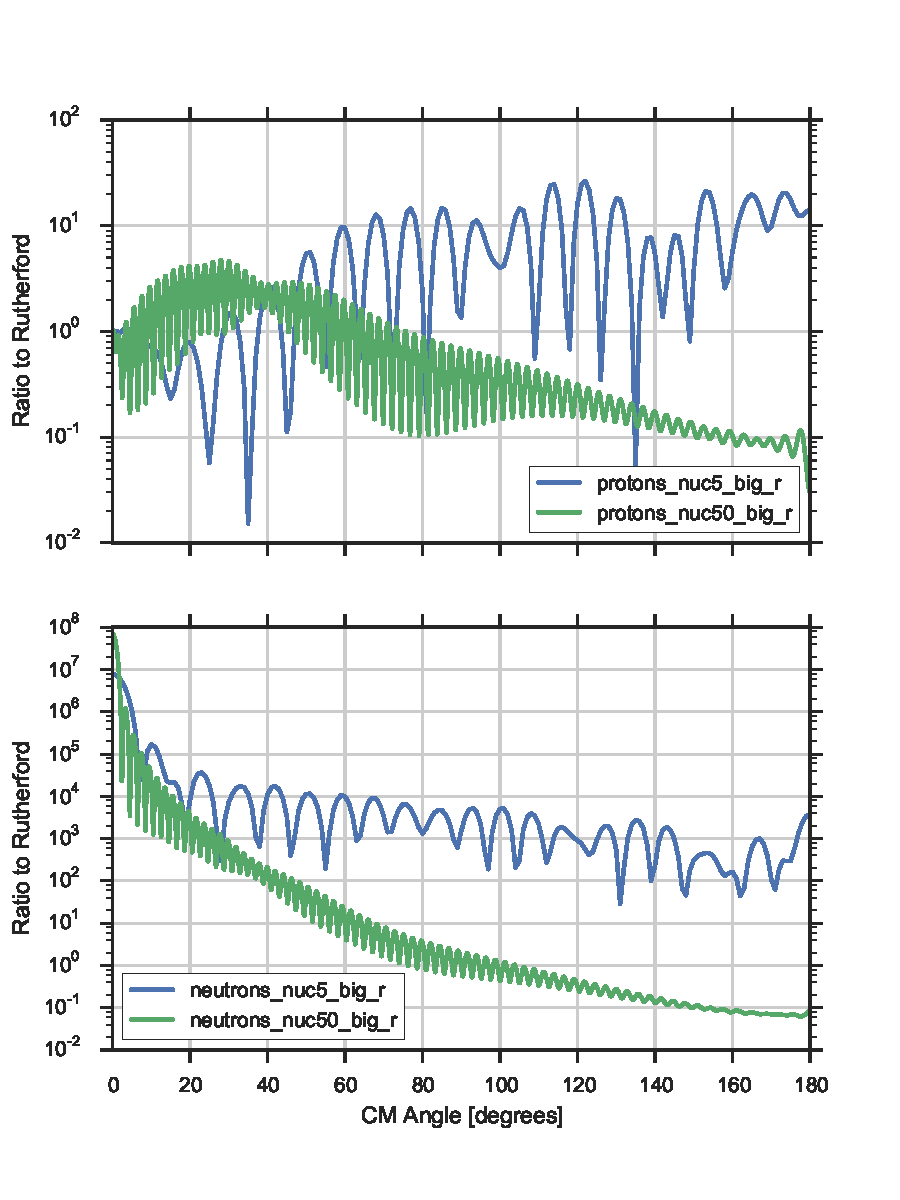
\includegraphics[width=\columnwidth]{{images/big_r.pdf}}
		\caption{Elastic scattering with the radius increased to \SI{10}{fm}.}
		\label{fig:big_r}
	\end{figure}

	\subsection{Total cross-sections}

	Finally, we found the total cross sections for neutron elastic scattering at our two energies. These are shown in Table~\ref{tab:xsec}.

	\begin{table}[h]
		\centering
		\begin{ruledtabular}
		\begin{tabular}{c c c c}
			Energy & Elastic & Absorption & Total \\
			\colrule
			\SI{5}{MeV}  & \SI{4843.87}{mb/sr} & \SI{426.24}{mb/sr} & \SI{5270.11}{mb/sr} \\
			\SI{50}{MeV} & \SI{2597.99}{mb/sr} & \SI{1567.59}{mb/sr} & \SI{4165.57}{mb/sr} \\
		\end{tabular}
		\end{ruledtabular}
		\caption{Neutron scattering cross sections from \fresco.}
		\label{tab:xsec}
	\end{table}


\section{Fitting experimental data}

Lorem ipsum \cite{Sakaguchi1982} Eiusmod id minim consequat pariatur cupidatat tempor officia in in labore sed irure quis anim commodo velit enim dolor anim laborum ad consectetur nostrud laboris veniam sed dolor ex commodo dolor cupidatat velit Ut est culpa eu ullamco proident eiusmod ut aliqua do esse ut dolor dolor laboris culpa consectetur enim Duis Excepteur et Duis cupidatat et qui dolore veniam dolore commodo voluptate Ut ad fugiat officia esse in eu commodo nostrud est officia id id ea qui amet sunt irure et consectetur occaecat aliquip ut velit ea labore dolore aliqua in proident do Duis tempor cillum pariatur aliqua aliquip in cupidatat et incididunt elit amet commodo consectetur quis Duis veniam proident exercitation occaecat anim in mollit Ut sunt dolore ut cillum Ut culpa officia consectetur nostrud culpa nisi sed laboris in nisi enim id dolor aliquip cupidatat laborum labore do Ut dolore exercitation occaecat dolore culpa magna culpa mollit in qui Duis laboris veniam Excepteur eiusmod nostrud minim dolor ullamco Ut officia Duis esse non ullamco qui consectetur cupidatat adipisicing nisi incididunt cillum et enim enim ad officia dolor eu laborum laboris mollit ea in Excepteur commodo officia tempor officia magna sint veniam qui proident sed aute Duis ea.

Lorem ipsum Ut in adipisicing deserunt ad laborum est aute esse cillum qui ad velit dolore aliqua irure proident in sint fugiat pariatur ullamco id incididunt non nulla incididunt Duis do ut enim aute aliqua mollit.

Lorem ipsum Eiusmod id minim consequat pariatur cupidatat tempor officia in in labore sed irure quis anim commodo velit enim dolor anim laborum ad consectetur nostrud laboris veniam sed dolor ex commodo dolor cupidatat velit Ut est culpa eu ullamco proident eiusmod ut aliqua do esse ut dolor dolor laboris culpa consectetur enim Duis Excepteur et Duis cupidatat et qui dolore veniam dolore commodo voluptate Ut ad fugiat officia esse in eu commodo nostrud est officia id id ea qui amet sunt irure et consectetur occaecat aliquip ut velit ea labore dolore aliqua in proident do Duis tempor cillum pariatur aliqua aliquip in cupidatat et incididunt elit amet commodo consectetur quis Duis veniam proident exercitation occaecat anim in mollit Ut sunt.

\begin{figure*}
	\centering
	\subfloat[Volume vs. Surface Potentials]{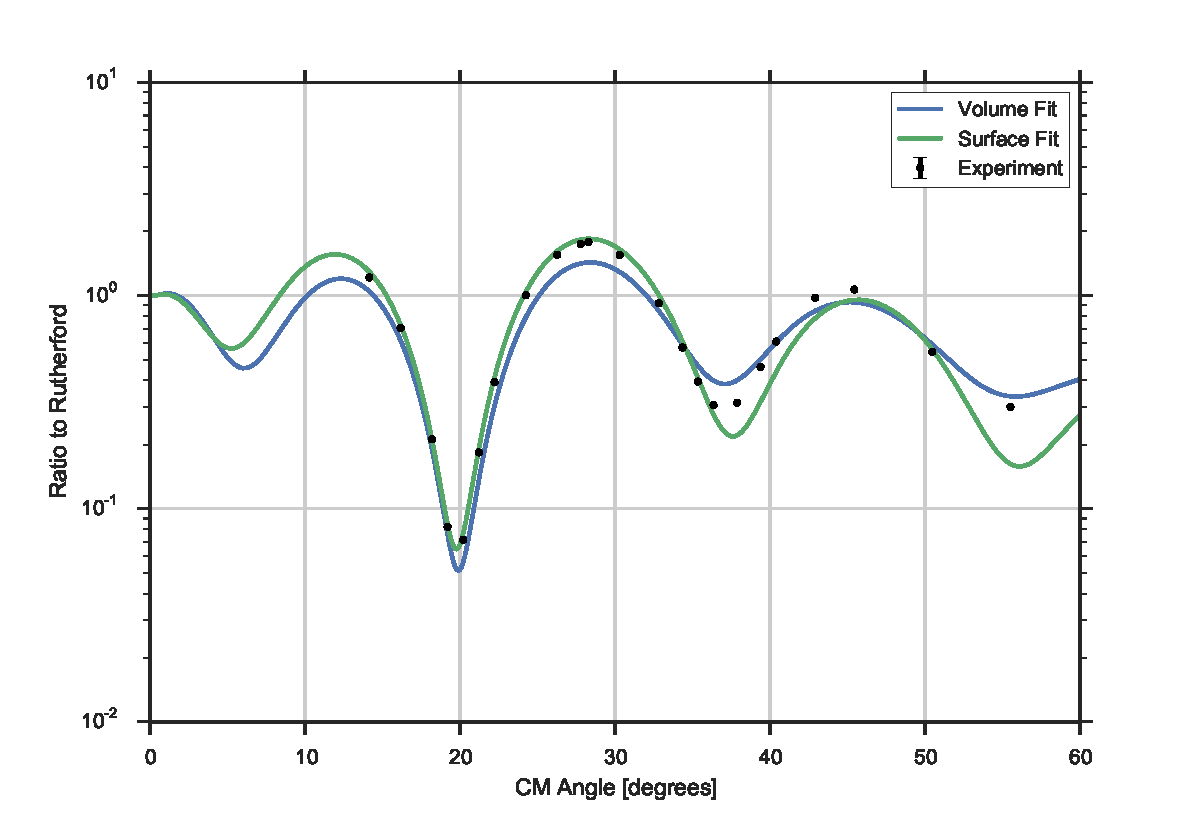
\includegraphics[width=\columnwidth]{images/vol_vs_surf.pdf}\label{fig:fits:a}}
	\subfloat[Surface with and without SO interaction]{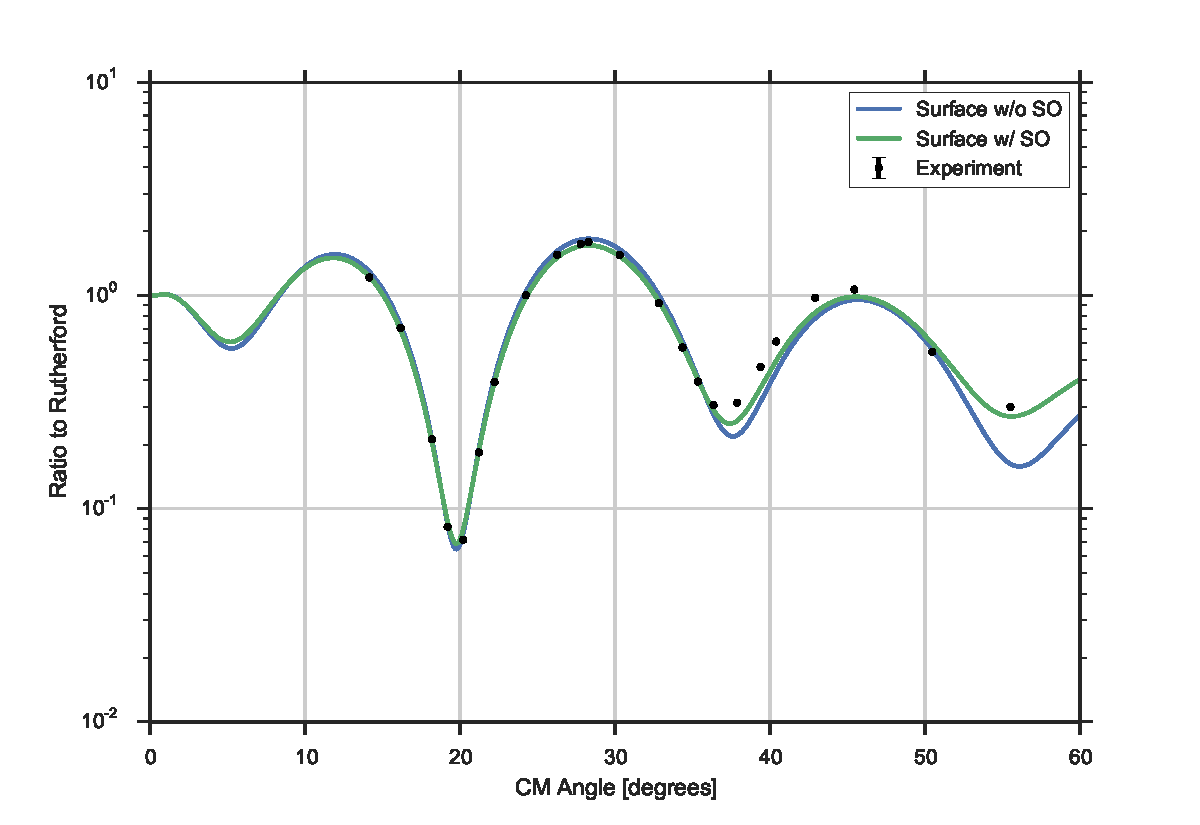
\includegraphics[width=\columnwidth]{images/surf_and_spin.pdf}\label{fig:fits:b}} \\
	\subfloat[Full fit vs. Surface+SO]{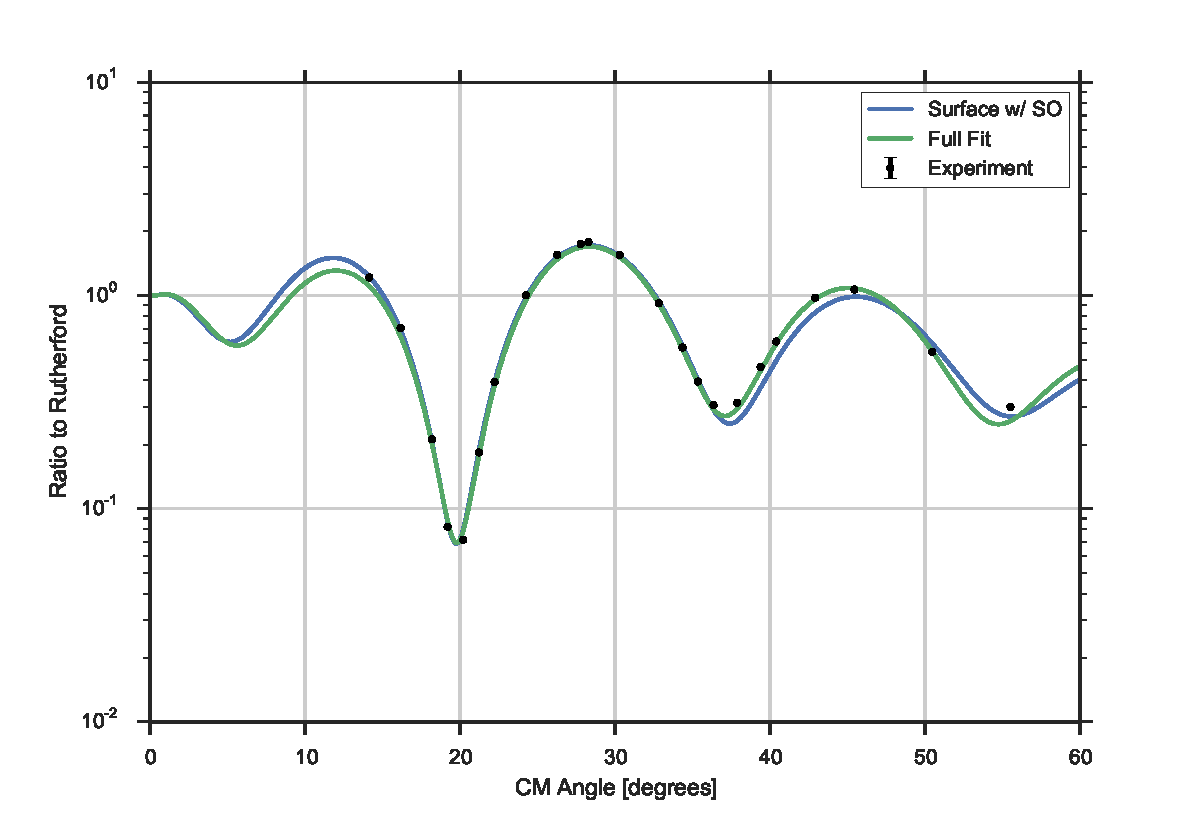
\includegraphics[width=\columnwidth]{images/everything_vs_surfso.pdf}\label{fig:fits:c}} 
	\subfloat[Full fit vs. Published Fit]{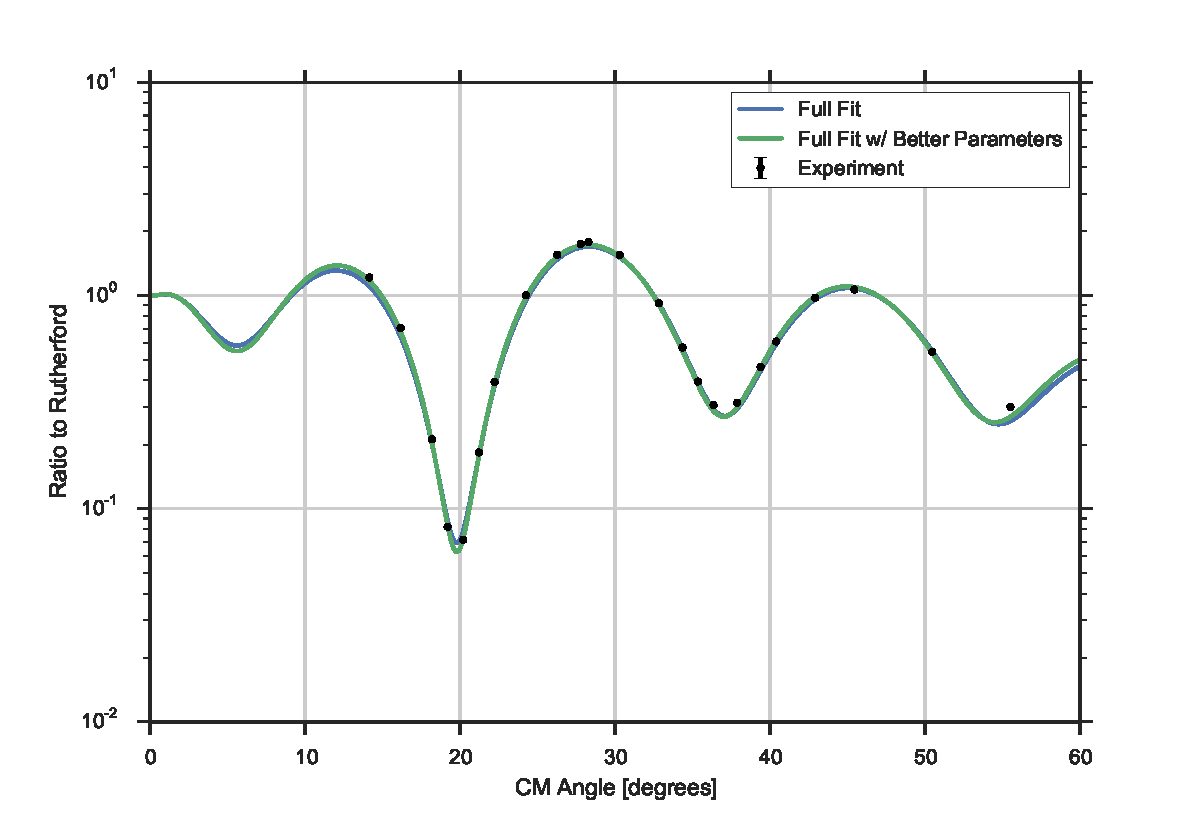
\includegraphics[width=\columnwidth]{images/comp_to_paper.pdf}\label{fig:fits:d}}
	\caption{Lorem ipsum Adipisicing quis pariatur consectetur nostrud reprehenderit dolor proident Duis do proident minim pariatur.}
	\label{fig:fits}
\end{figure*}

\bibliography{hw2}

\end{document}